\documentclass[a4paper]{article}
\usepackage[utf8]{inputenc}
\usepackage[russian]{babel}
\usepackage[margin=1in]{geometry}
\usepackage{float}
\usepackage{graphicx}
\usepackage{setspace}
\usepackage{indentfirst}
\title{Лабораторная работа}
\author{Шулайкин Д.А.}
\begin{document}
\onehalfspacing
\thispagestyle{empty}
\begin{center}
Министерство образования и науки Российской Федерации
\vspace{10pt}

Федеральное государственное бюджетное образовательное учереждение высшего образования "Ивановский государственный энергетический университет имени В.И. Ленина"
\vspace{40pt}

Кафедра ПОКС
\vspace{40pt}

\textbf{Отчет по лабораторной работе №1}

Дисциплина: ``АРХИТЕКТУРА ВЫЧИСЛИТЕЛЬНЫХ СИСТЕМ''

Тема: ``ИЗУЧЕНИЕ АППАРАТНЫХ СРЕДСТВ ЭВМ''

\end{center}

\vspace{330pt}
\begin{flushright}
\textbf{Выполнили:} \\
ст. гр. $2-42В_{xx}$ \\
Шулайкин Д.А. \\
Ужастин К.А. \\

\textbf{Проверил:} \\
ст. преп. Наумов Ю.В.

\end{flushright}
\vspace{40pt}
\begin{center}
Иваново 2018
\end{center}
\pagebreak

\section{Цель работы} Изучить составные части персонального компьютера(процессор, материнская плата, видеокарта, ОЗУ, HDD, FDD, CD-ROM, звуковая карта на примере персонального компьютера); научиться разбираться в строении персонального компьютера, разобрать и собрать системный блок. 

\section{Задание к лабораторной работе}
\begin{enumerate}
\item Выполнить разборку и сборку системного блока ЭВМ. 
\item Выполнить описание и изучить основные характеристики аппаратных средств ЭВМ.
\end{enumerate}

\section{Ход работы}
\begin{enumerate}
    \item Изучить теоретический материал, записав основные моменты лабораторной работы.
    \item отвернуть винты, снять кожух системного блока ЭВМ; 
    \item отключить кабели питания и шлейфы жесткого диска, демонтировать жесткий диск;
    \item отключить кабели питания и шлейфы привода CD-ROM, демонтировать привод СD-ROM;
    \item отключить кабели питания и шлейфы FDD-дисковода, демонтировать дисковод;
    \item демонтировать блок питания
    \item демонтировать сетевую карту
    \item демонтировать видеокарту
    \item демонтировать панель с материнской платой из корпуса
    \item демонтировать материнскую плату
    \item демонтировать платы памяти
    \item демонтировать вентилятор и радиатор с процессора
    \item демонтировать процессор
    \item замонтировать все в обратном порядке
\end{enumerate}

\begin{table}[ht]
\centering
\begin{tabular}{|l|l|c|}
\hline
№ п/п & Тип устройства & Модель устройства\\
\hline
1 & Материнская плата & Gigabyte GA-8ST800 \\
2 & Центральный процессор & Intel Pentium 4 HT\\
3 & ОЗУ & SAMSUNG DDR DIMM 512Mb\\
4 & НЖМД & Seagate Barracuda ST340014A \\ 
5 & Видеокарта & NVIDIA GeForce 4 MX 440-8x \\
6 & Звуковая карта & Genius Sound Maker 32X \\
7 & Оптический носитель & TEAC CD-W54E \\ 
8 & Сетевой адаптер & Intel Fast E-net\\
9 & Блок питания & Macropower MP-340AR\\
\hline
\end{tabular}
\end{table}

\subsection{Материнская плата}
\subsubsection{Фото}
\begin{figure}[H]
\centering
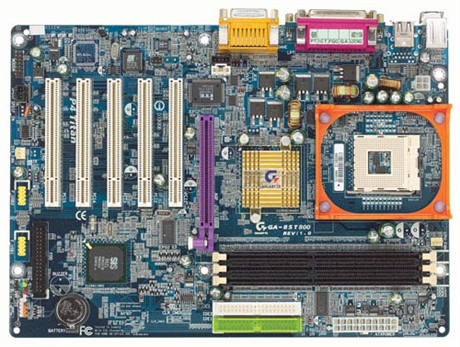
\includegraphics[scale=0.5]{motherboard.jpg} 
\end{figure}
\subsubsection{Характеристики}
\begin{table}[H]
    \centering
    \begin{tabular}{|l|l|}
    \hline
    Характеристика & Значение \\
    \hline
    Чипсет & SiS645DX \\
    Сокет & 478 \\
    Слоты расширеняи & 3x DIMM 184-pin, 1 x AGP 4x, 5 x PCI \\
    Внешние порты & 4x USB 2.0, 1x PS/2 keyboard, 1x PS/2 mouse, 2x serial, 1x parallel \\
    Внутренние интерфейсы & ATA-133 connectors: 2x 40pin IDC, 1x floppy \\
    Форм-фактор & ATX \\
    \hline
\end{tabular}
\end{table}
    
\subsection{Процессор}
\subsubsection{Фото}
\begin{figure}[H]
\centering
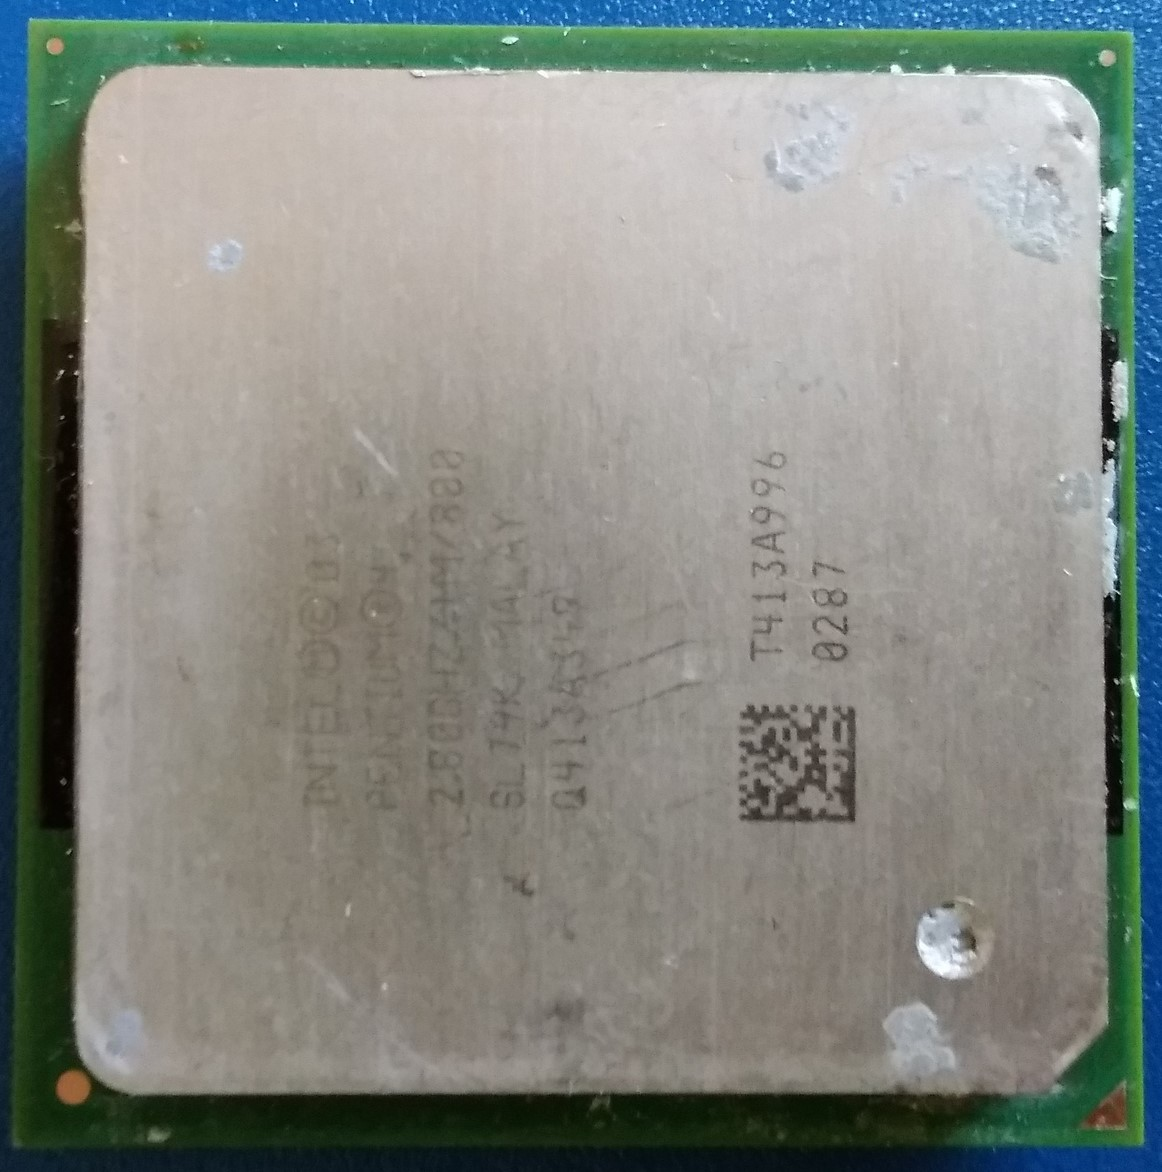
\includegraphics[scale=0.1]{cpu.jpg} 
\end{figure}

\subsubsection{Характеристики}
\begin{table}[H]
\centering
\begin{tabular}{|l|l|}
    \hline
    Характеристика & Значение \\
    \hline
    Тактовая частота & 2.8 Ghz \\
    Socket & 478 \\ 
    Cache L2 & 512 KB \\
    \hline
\end{tabular}
\end{table}

\subsection{ОЗУ}
\subsubsection{Фото}
\begin{figure}[H]
\centering
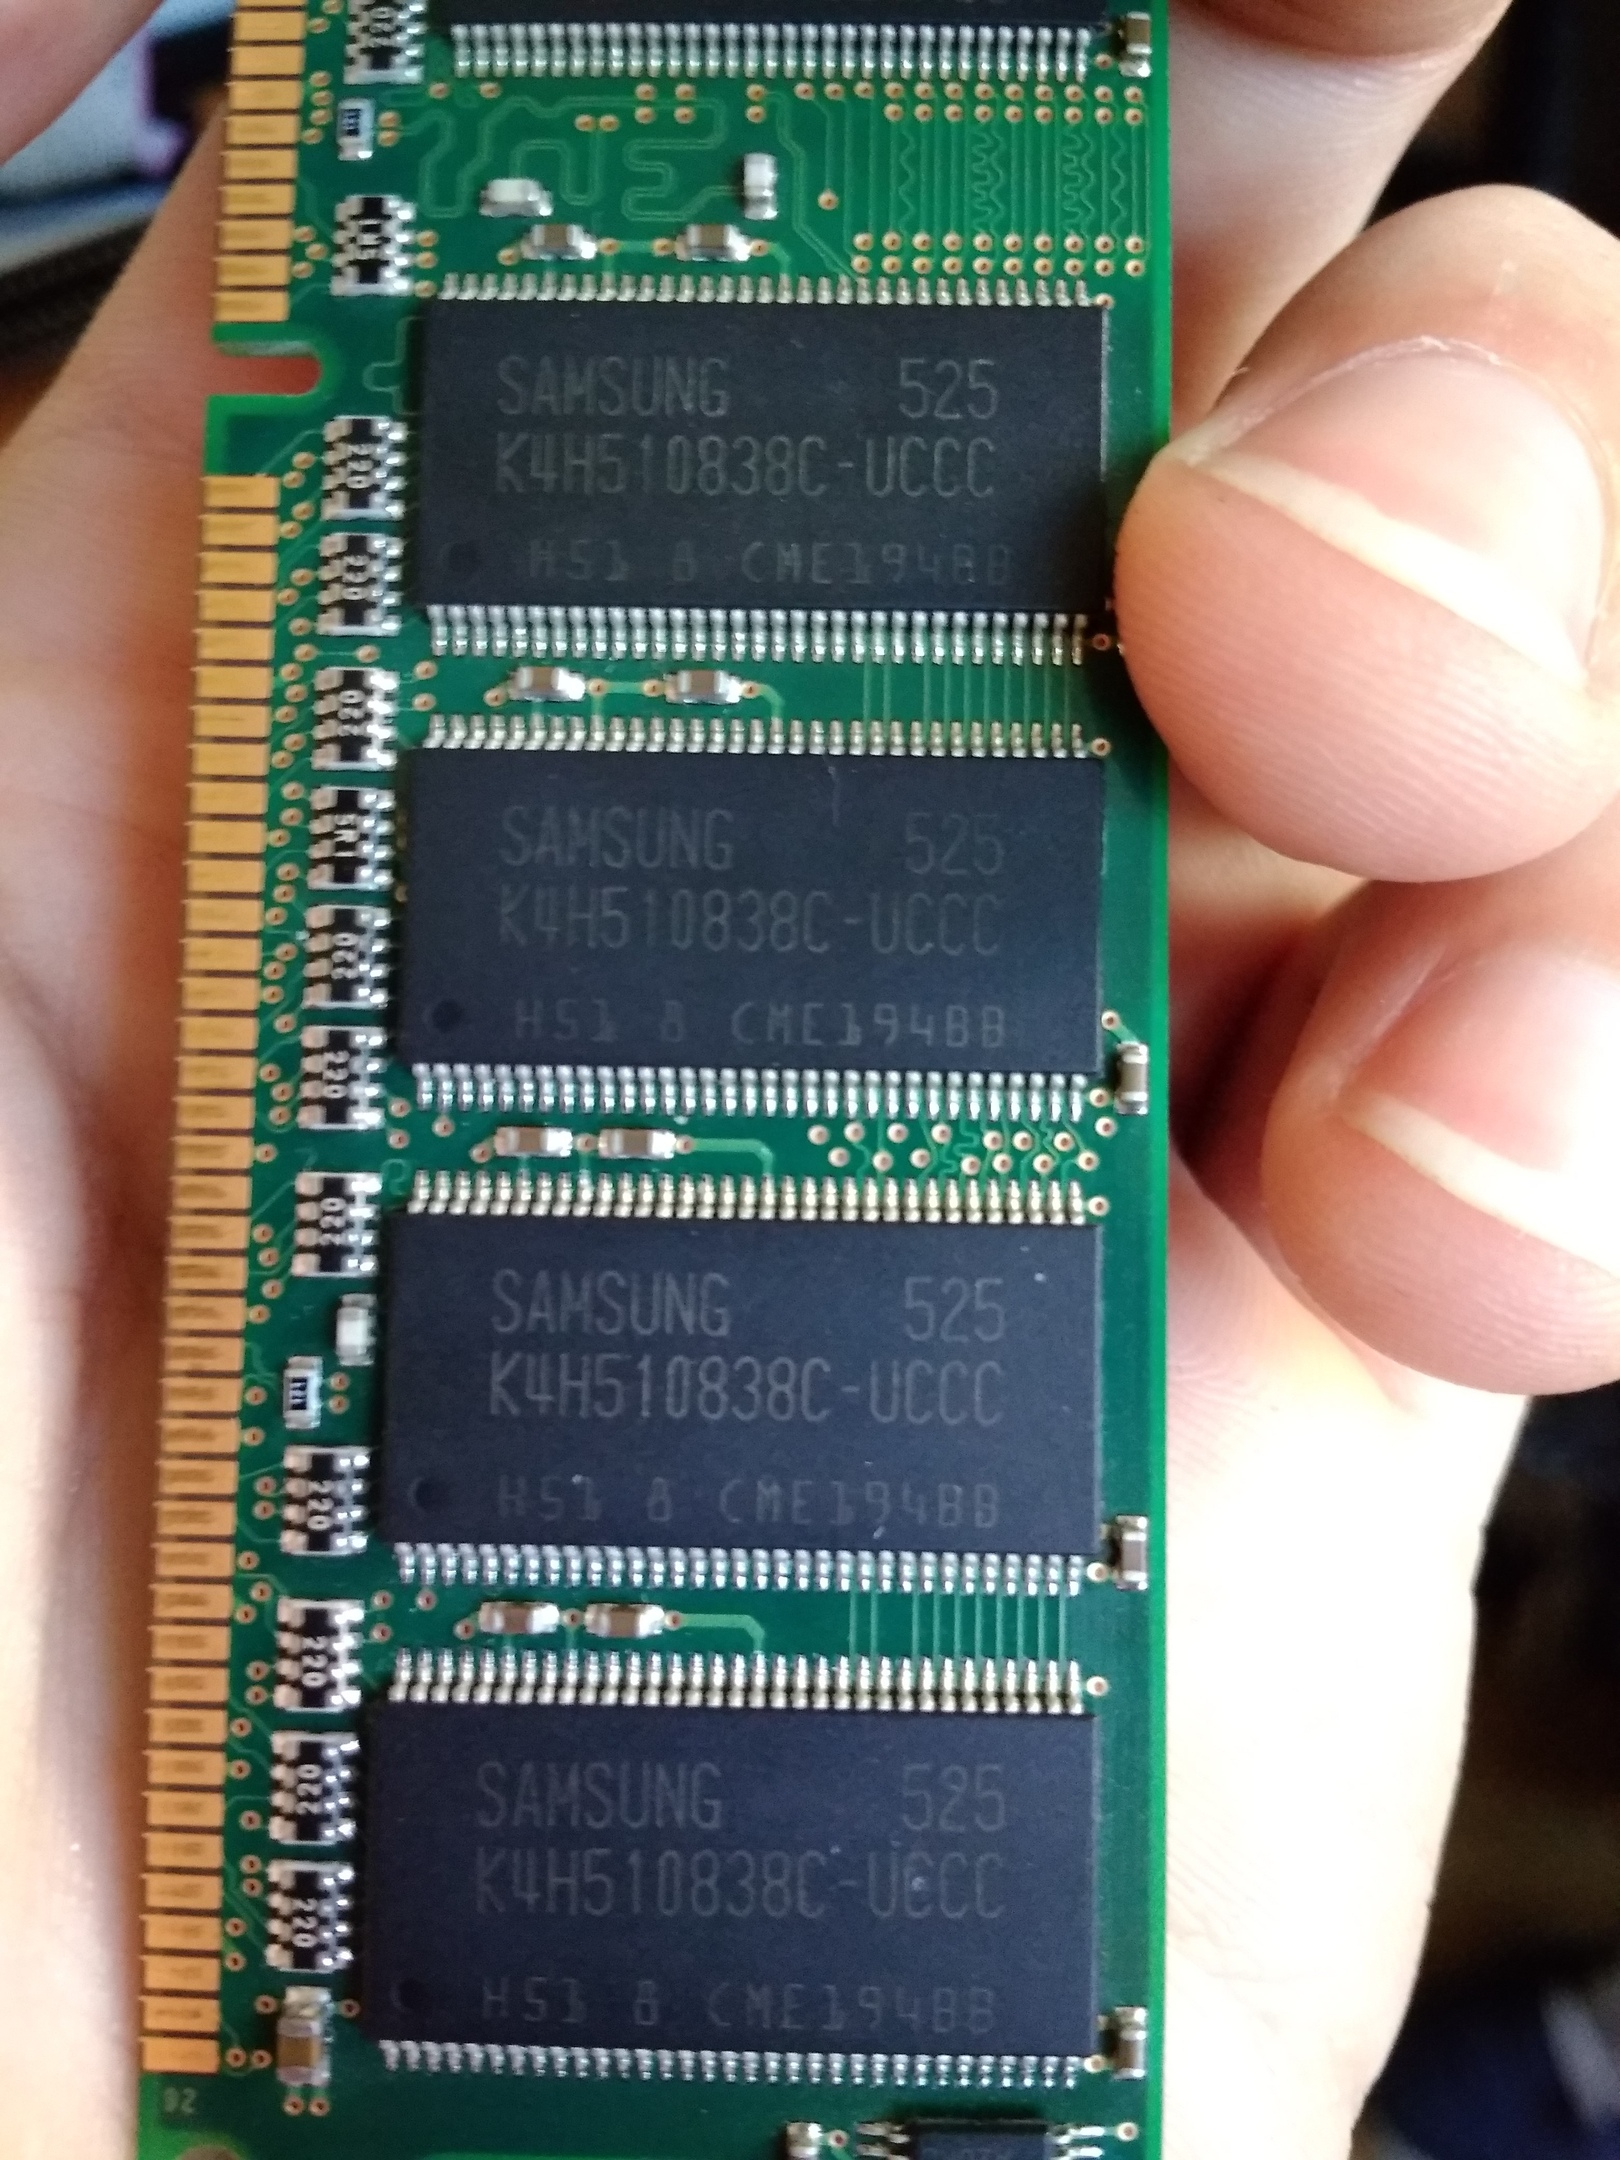
\includegraphics[scale=0.1]{ram.jpg} 
\end{figure}
\subsubsection{Характеристики}
\begin{table}[H]
    \centering
    \begin{tabular}{|l|l|}
    \hline
    Характеристика & Значение \\
    \hline
    Количество модулей & 1x \\
    Объем & 512 Mb \\
    Тип памяти & PC-3200 (DDR SDRAM 400 Mhz) \\
    \hline
\end{tabular}
\end{table}

\subsection{НЖМД}
\subsubsection{Фото}
\begin{figure}[H]
\centering
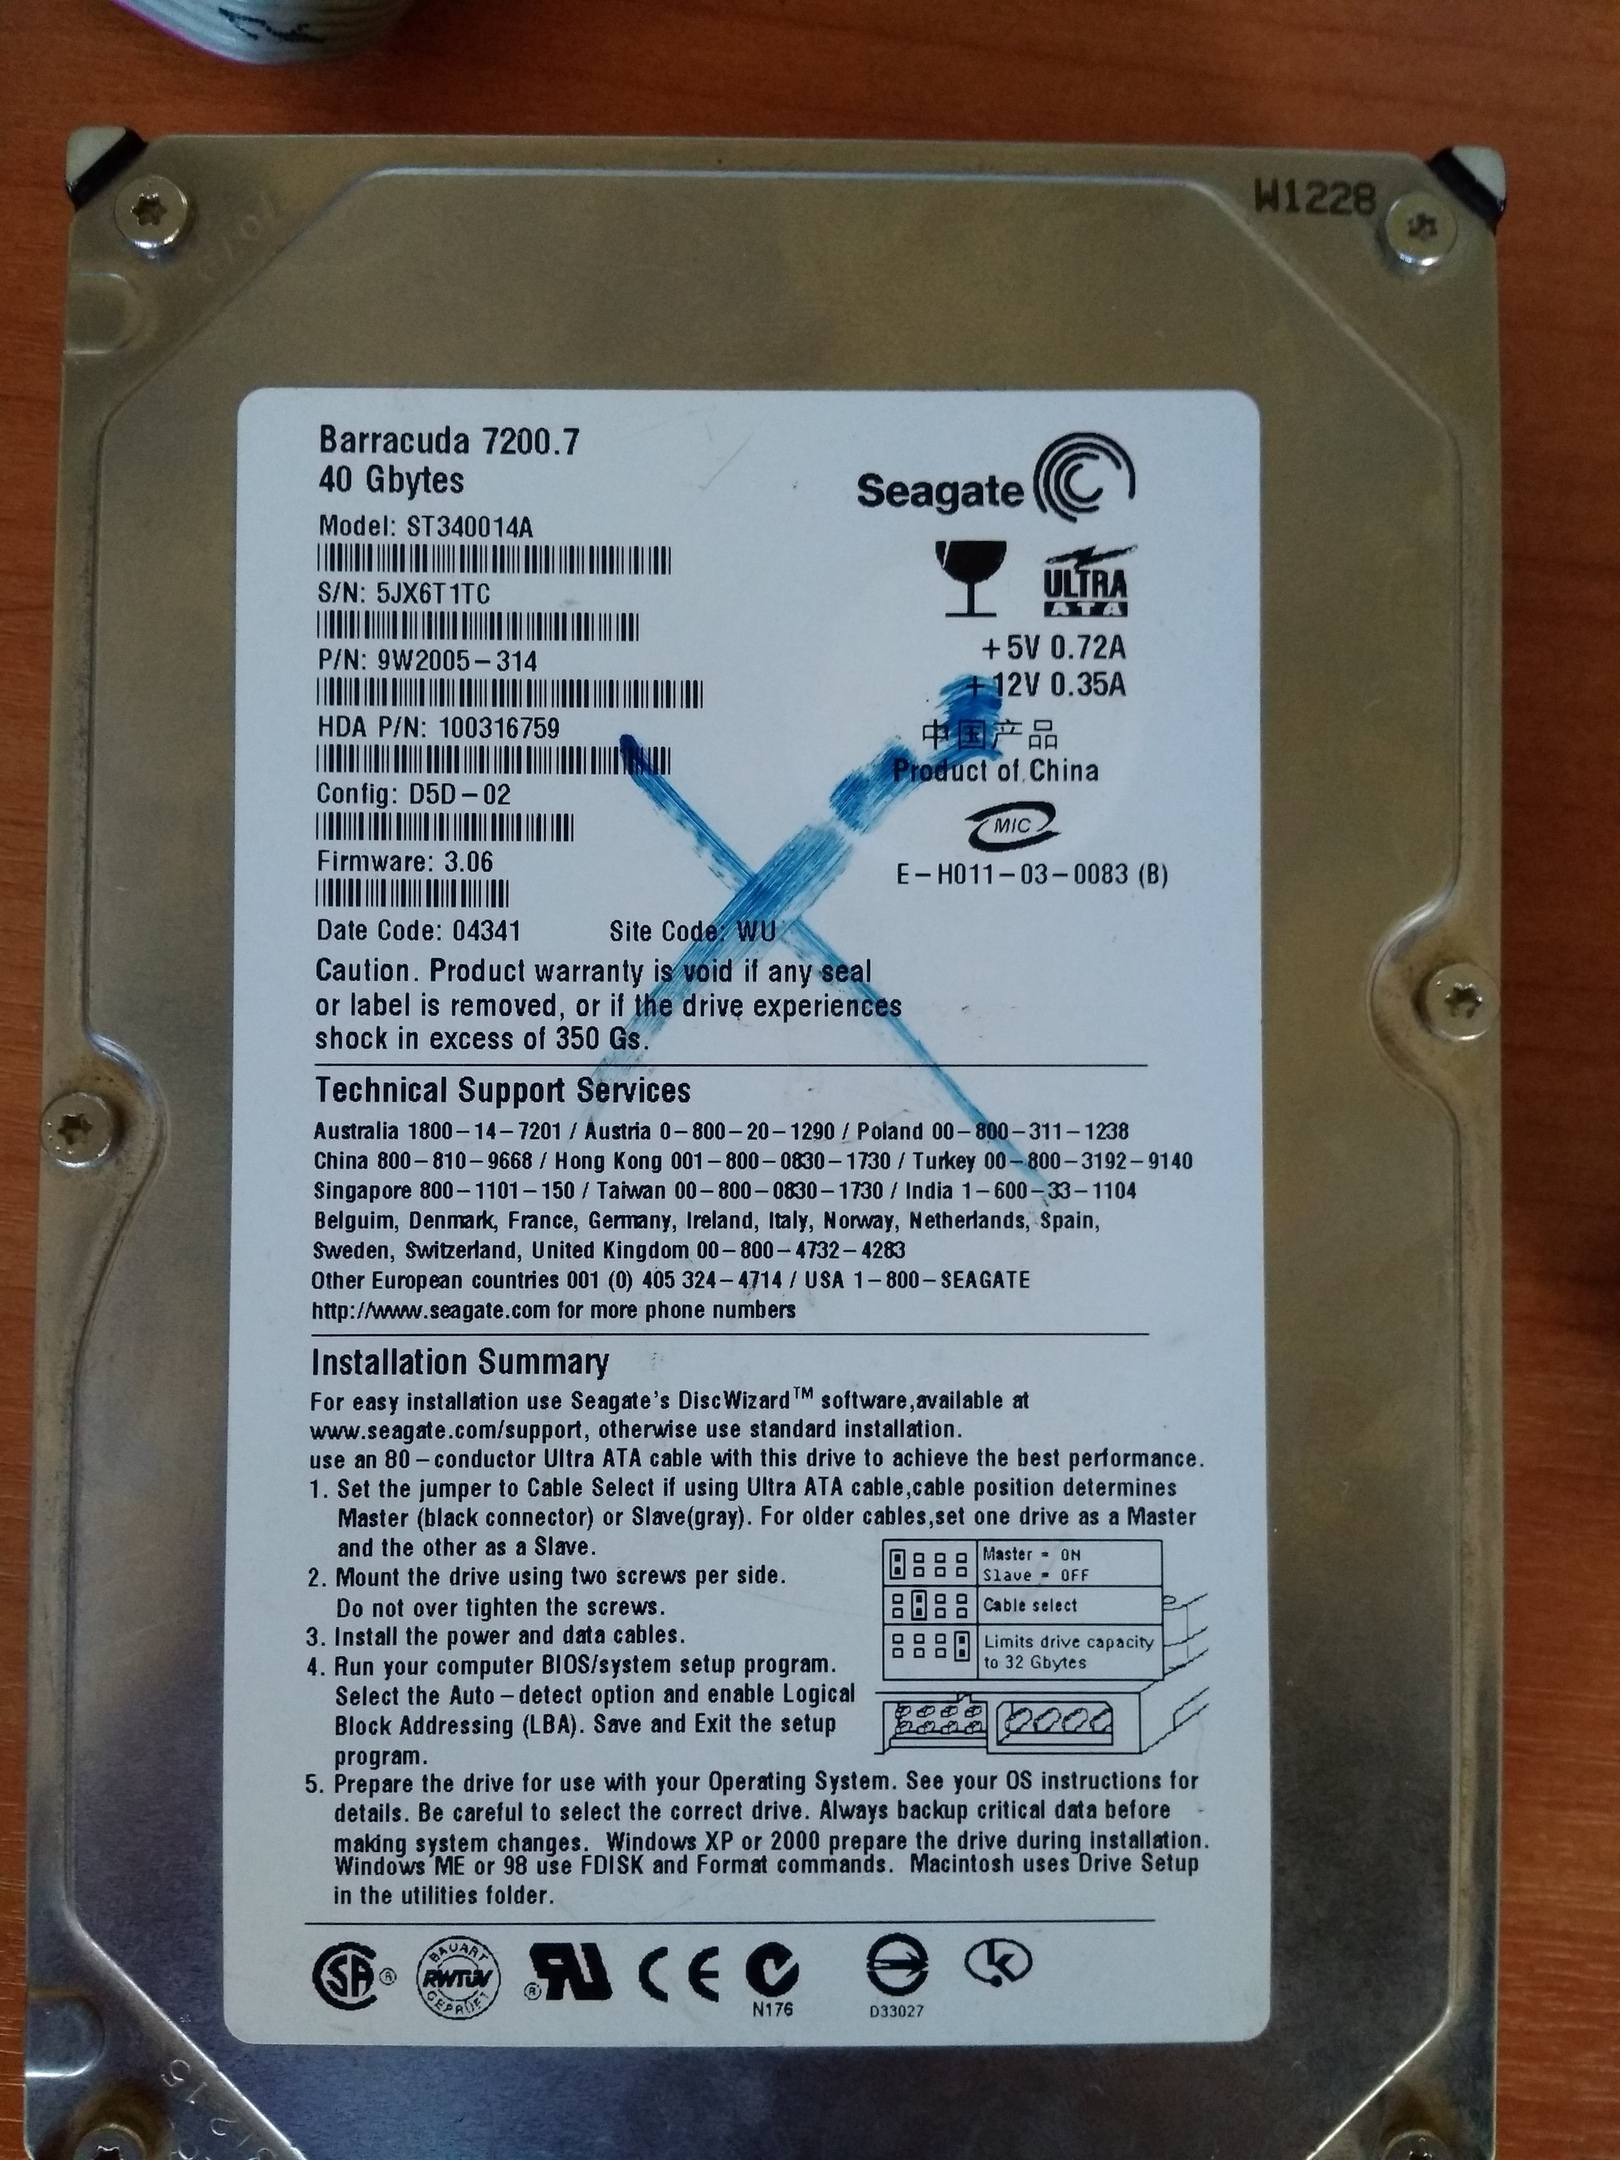
\includegraphics[scale=0.1]{harddrive.jpg} 
\end{figure}
\subsubsection{Характеристики}
\begin{table}[H]
    \centering
    \begin{tabular}{|l|l|}
    \hline
    Характеристика & Значение \\
    \hline
    Емкость накопителя & 40Gb \\
    Скорость вращения шпинделя & 7200Rpm \\
    Buffer size & 2 Mb \\
    интерфейс & IDE \\
    Форм-фактор & 3.5'' \\
    \hline
\end{tabular}
\end{table}

\subsection{Видеокарта}
\subsubsection{Фото}
\begin{figure}[H]
\centering
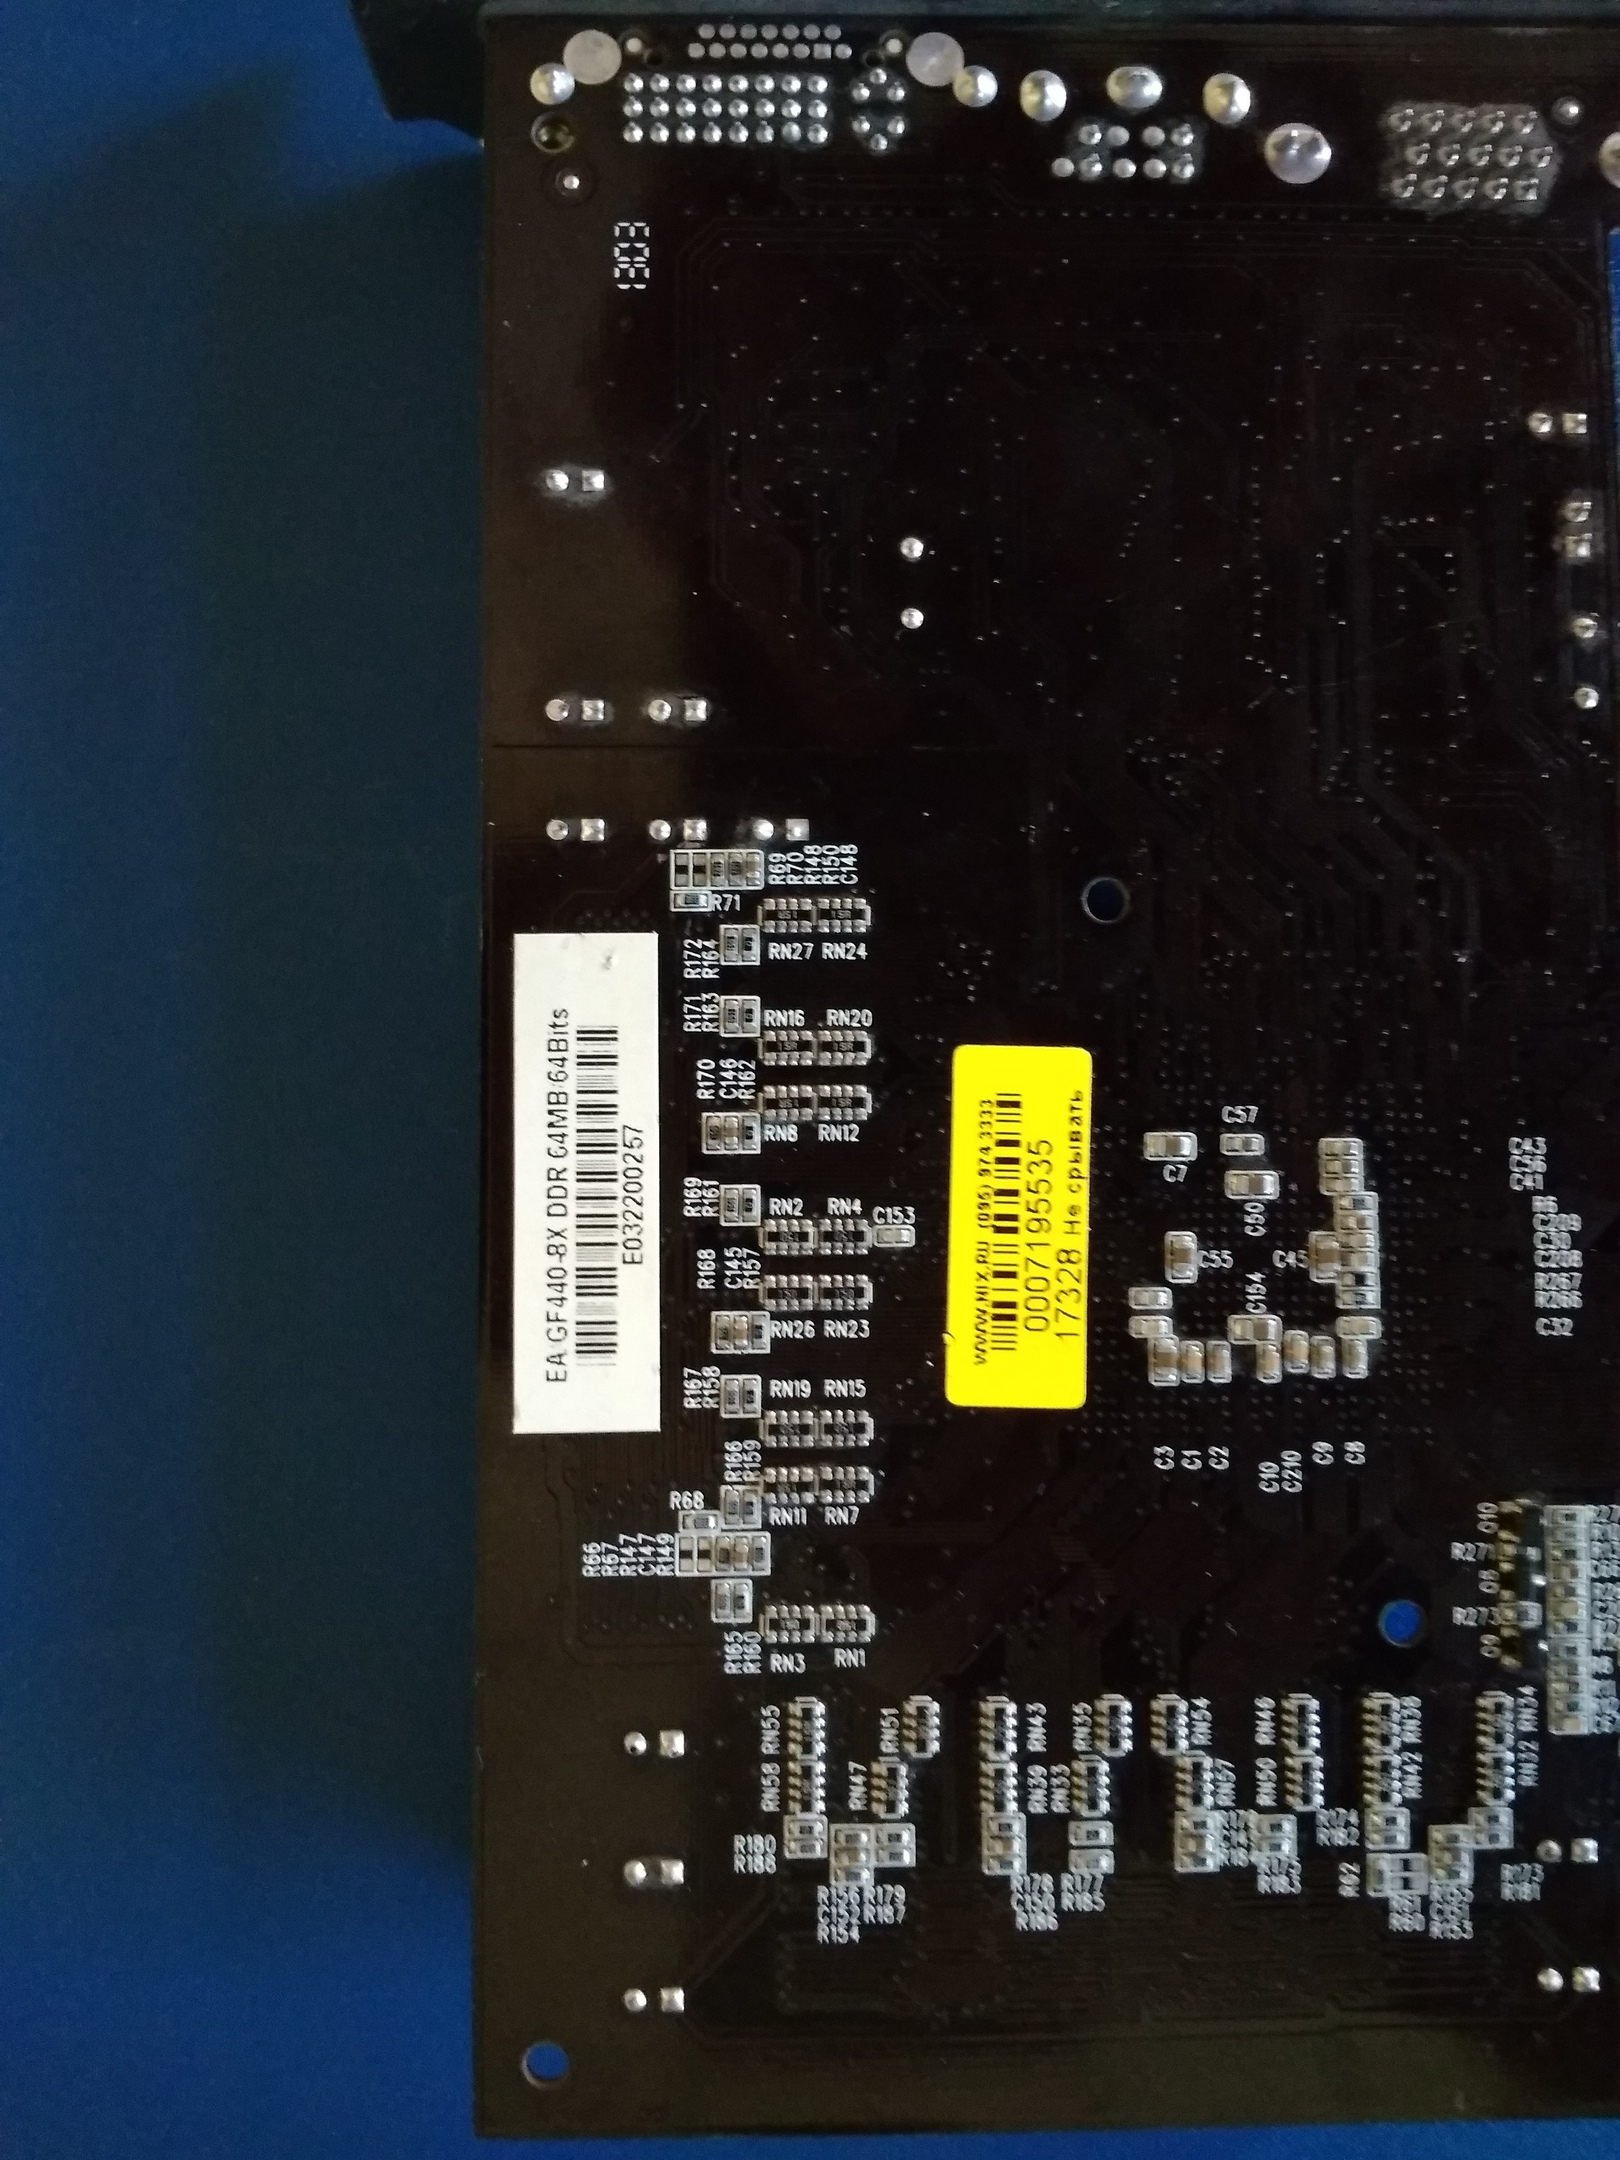
\includegraphics[scale=0.1]{gpu.jpg} 
\end{figure}
\subsubsection{Характеристики}
\begin{table}[H]
    \centering
    \begin{tabular}{|l|l|}
    \hline
    Характеристика & Значение \\
    \hline
    RAMDAC & 350Mhz \\
    Объем видеопамяти & 64Mb \\
    Тип видеопамяти & DDR SDRAM \\
    Интерфейс & AGP \\
    Порты & 15pin D-Sub, DVI-I \\
    \hline
\end{tabular}
\end{table}

\subsection{Звуковая карта}
\subsubsection{Фото}
\begin{figure}[H]
\centering
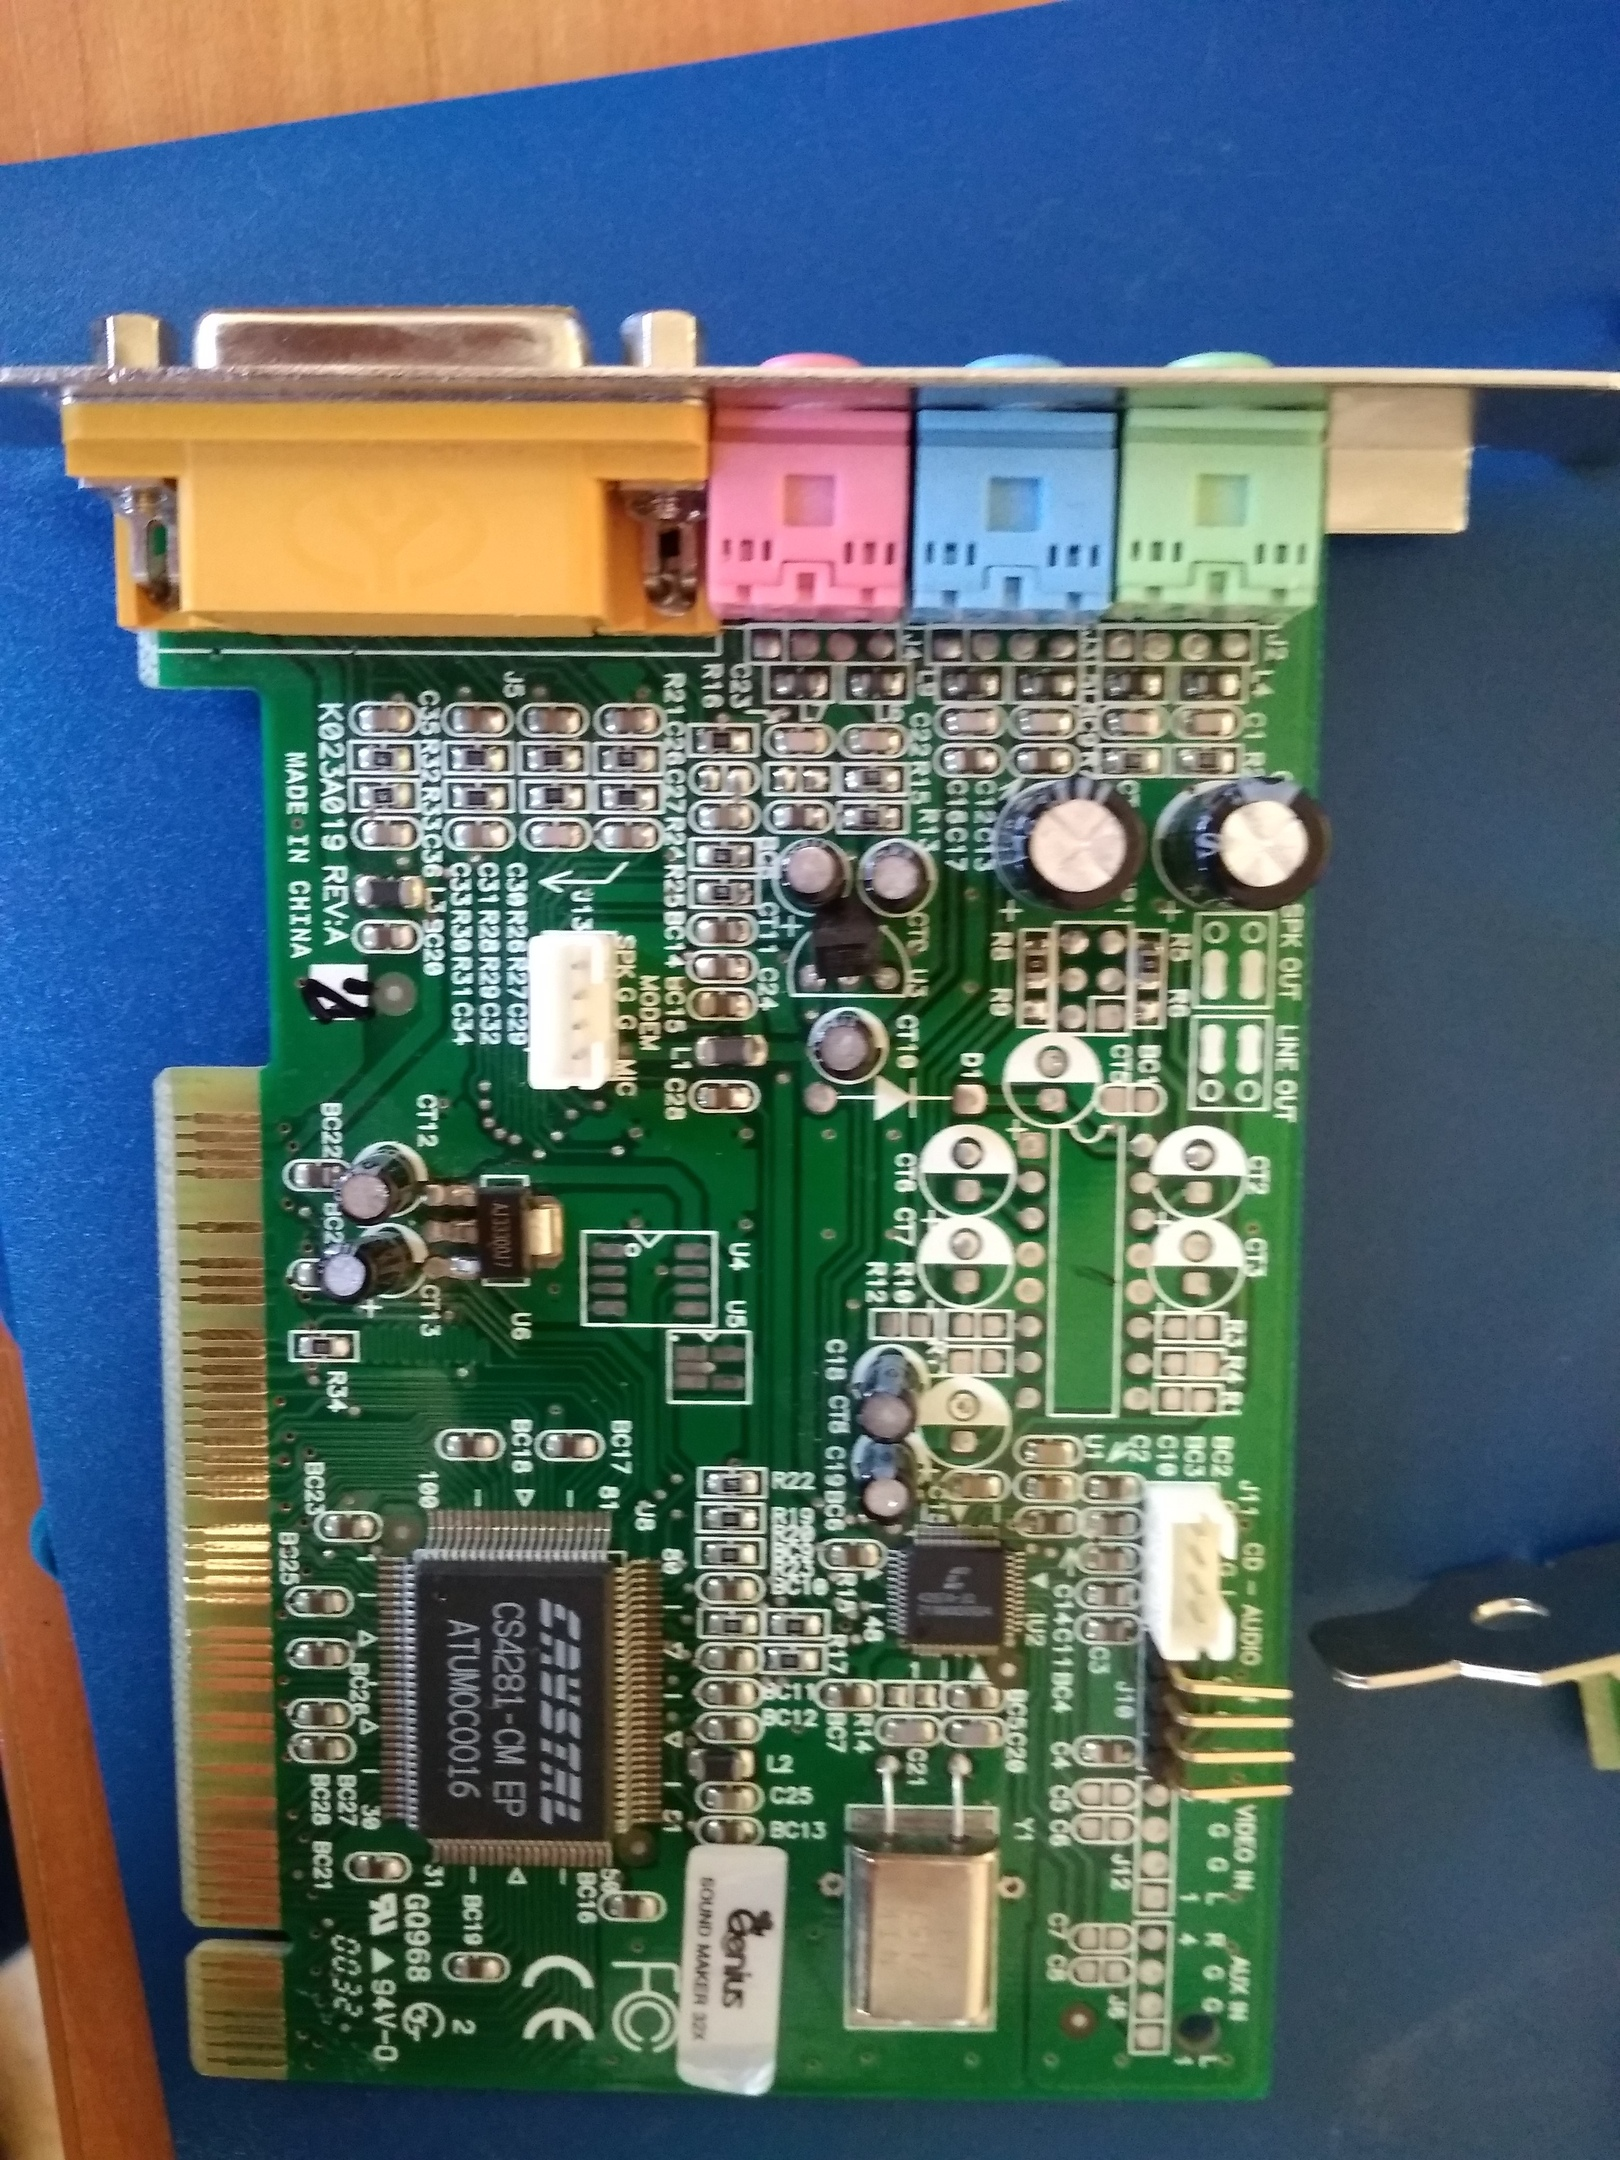
\includegraphics[scale=0.1]{sc.jpg} 
\end{figure}
\subsubsection{Характеристики}
\begin{table}[H]
    \centering
    \begin{tabular}{|l|l|}
    \hline
    Характеристика & Значение \\
    \hline
    Интерфейс & PCI \\
    Порты & Audio line-in, Microphone, Audio out,  1x gameport/MIDI \\
    \hline
\end{tabular}
\end{table}

\subsection{Оптический носитель}
\subsubsection{Фото}
\begin{figure}[H]
\centering
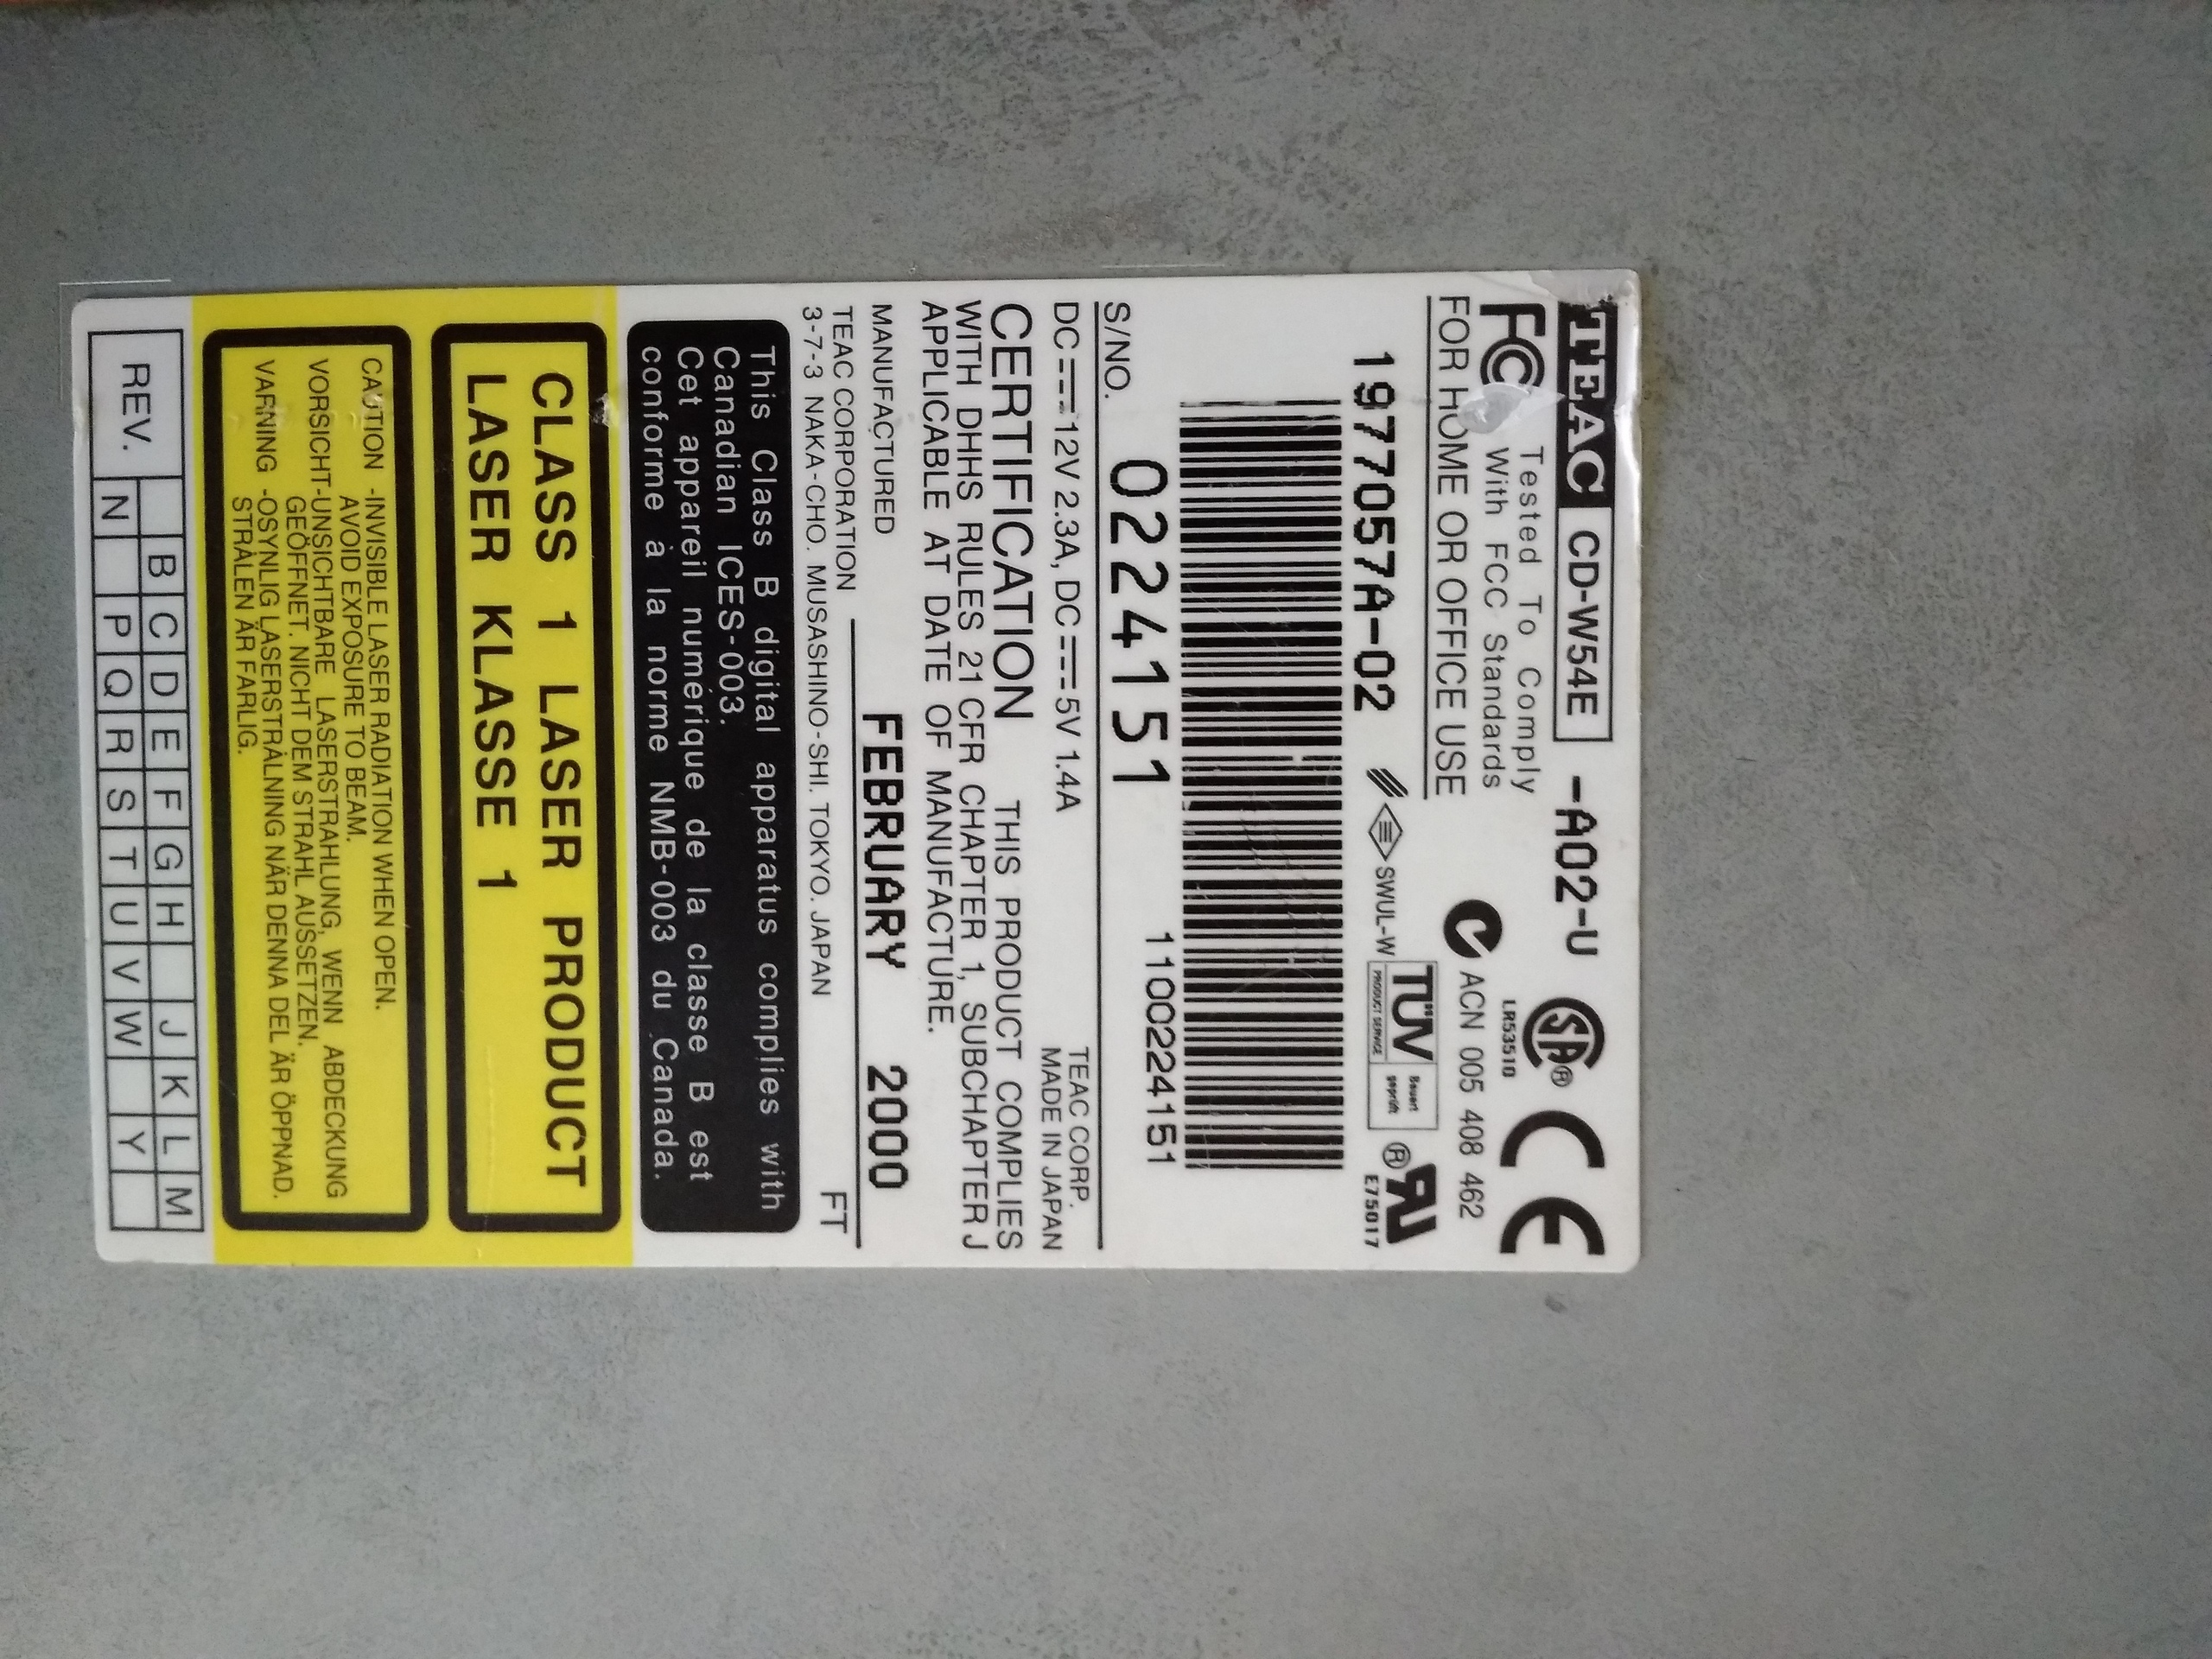
\includegraphics[scale=0.1]{cd.jpg} 
\end{figure}
\subsubsection{Характеристики}
\begin{table}[H]
    \centering
    \begin{tabular}{|l|l|}
    \hline
    Характеристика & Значение \\
    \hline
    Compliant Standards & CD-DA, CD-XA, CDi, Kodak PhotoCD \\
    Read Speed & 32x \\
    Write Speed & 4x \\
    Rewrite Speed & 4x \\
    Форм фактор & 5.25" x 1/2H \\
    Интерфейс & IDE \\
    \hline
\end{tabular}
\end{table}

\subsection{Сетевой адаптер}
\subsubsection{Фото}
\begin{figure}[H]
\centering
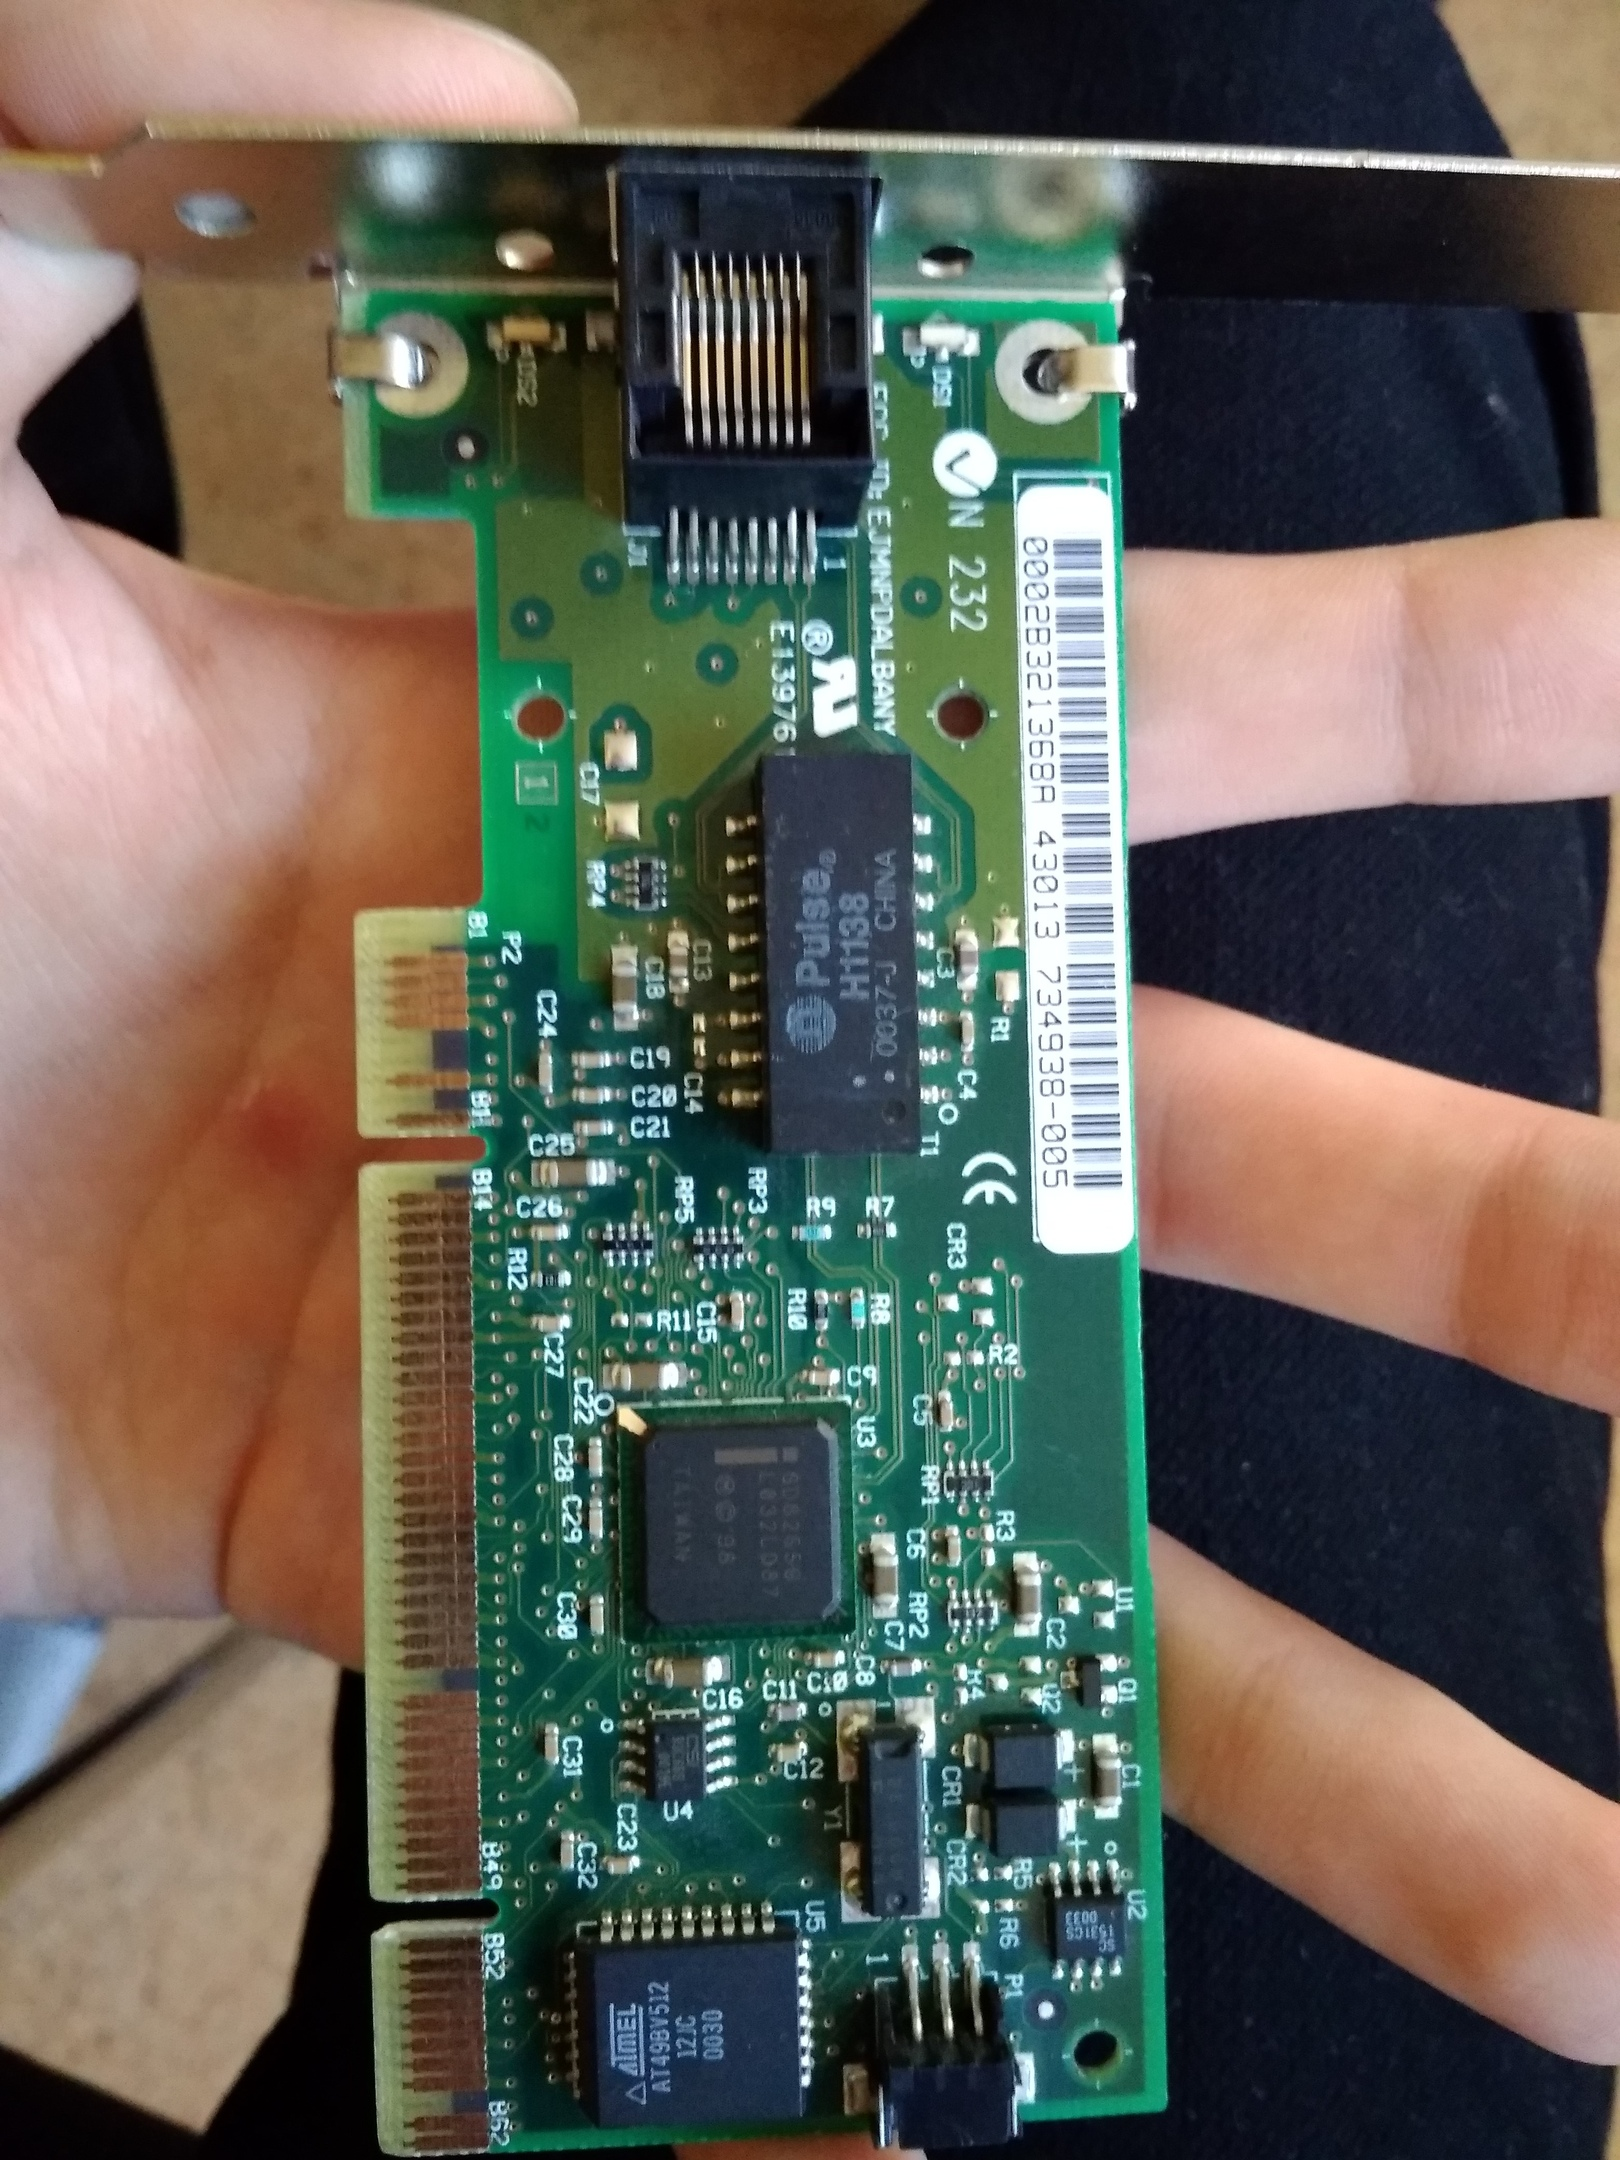
\includegraphics[scale=0.1]{nc.jpg} 
\end{figure}
\subsubsection{Характеристики}
\begin{table}[H]
\centering
\begin{tabular}{|l|l|}
\hline
Характеристика & Значение \\
\hline
Интерфейс & PCI \\
Порты & 1x Ethernet 100Mbps \\
\hline
\end{tabular}
\end{table}

\subsection{Блок питания}
\subsubsection{Фото}
\begin{figure}[H]
\centering
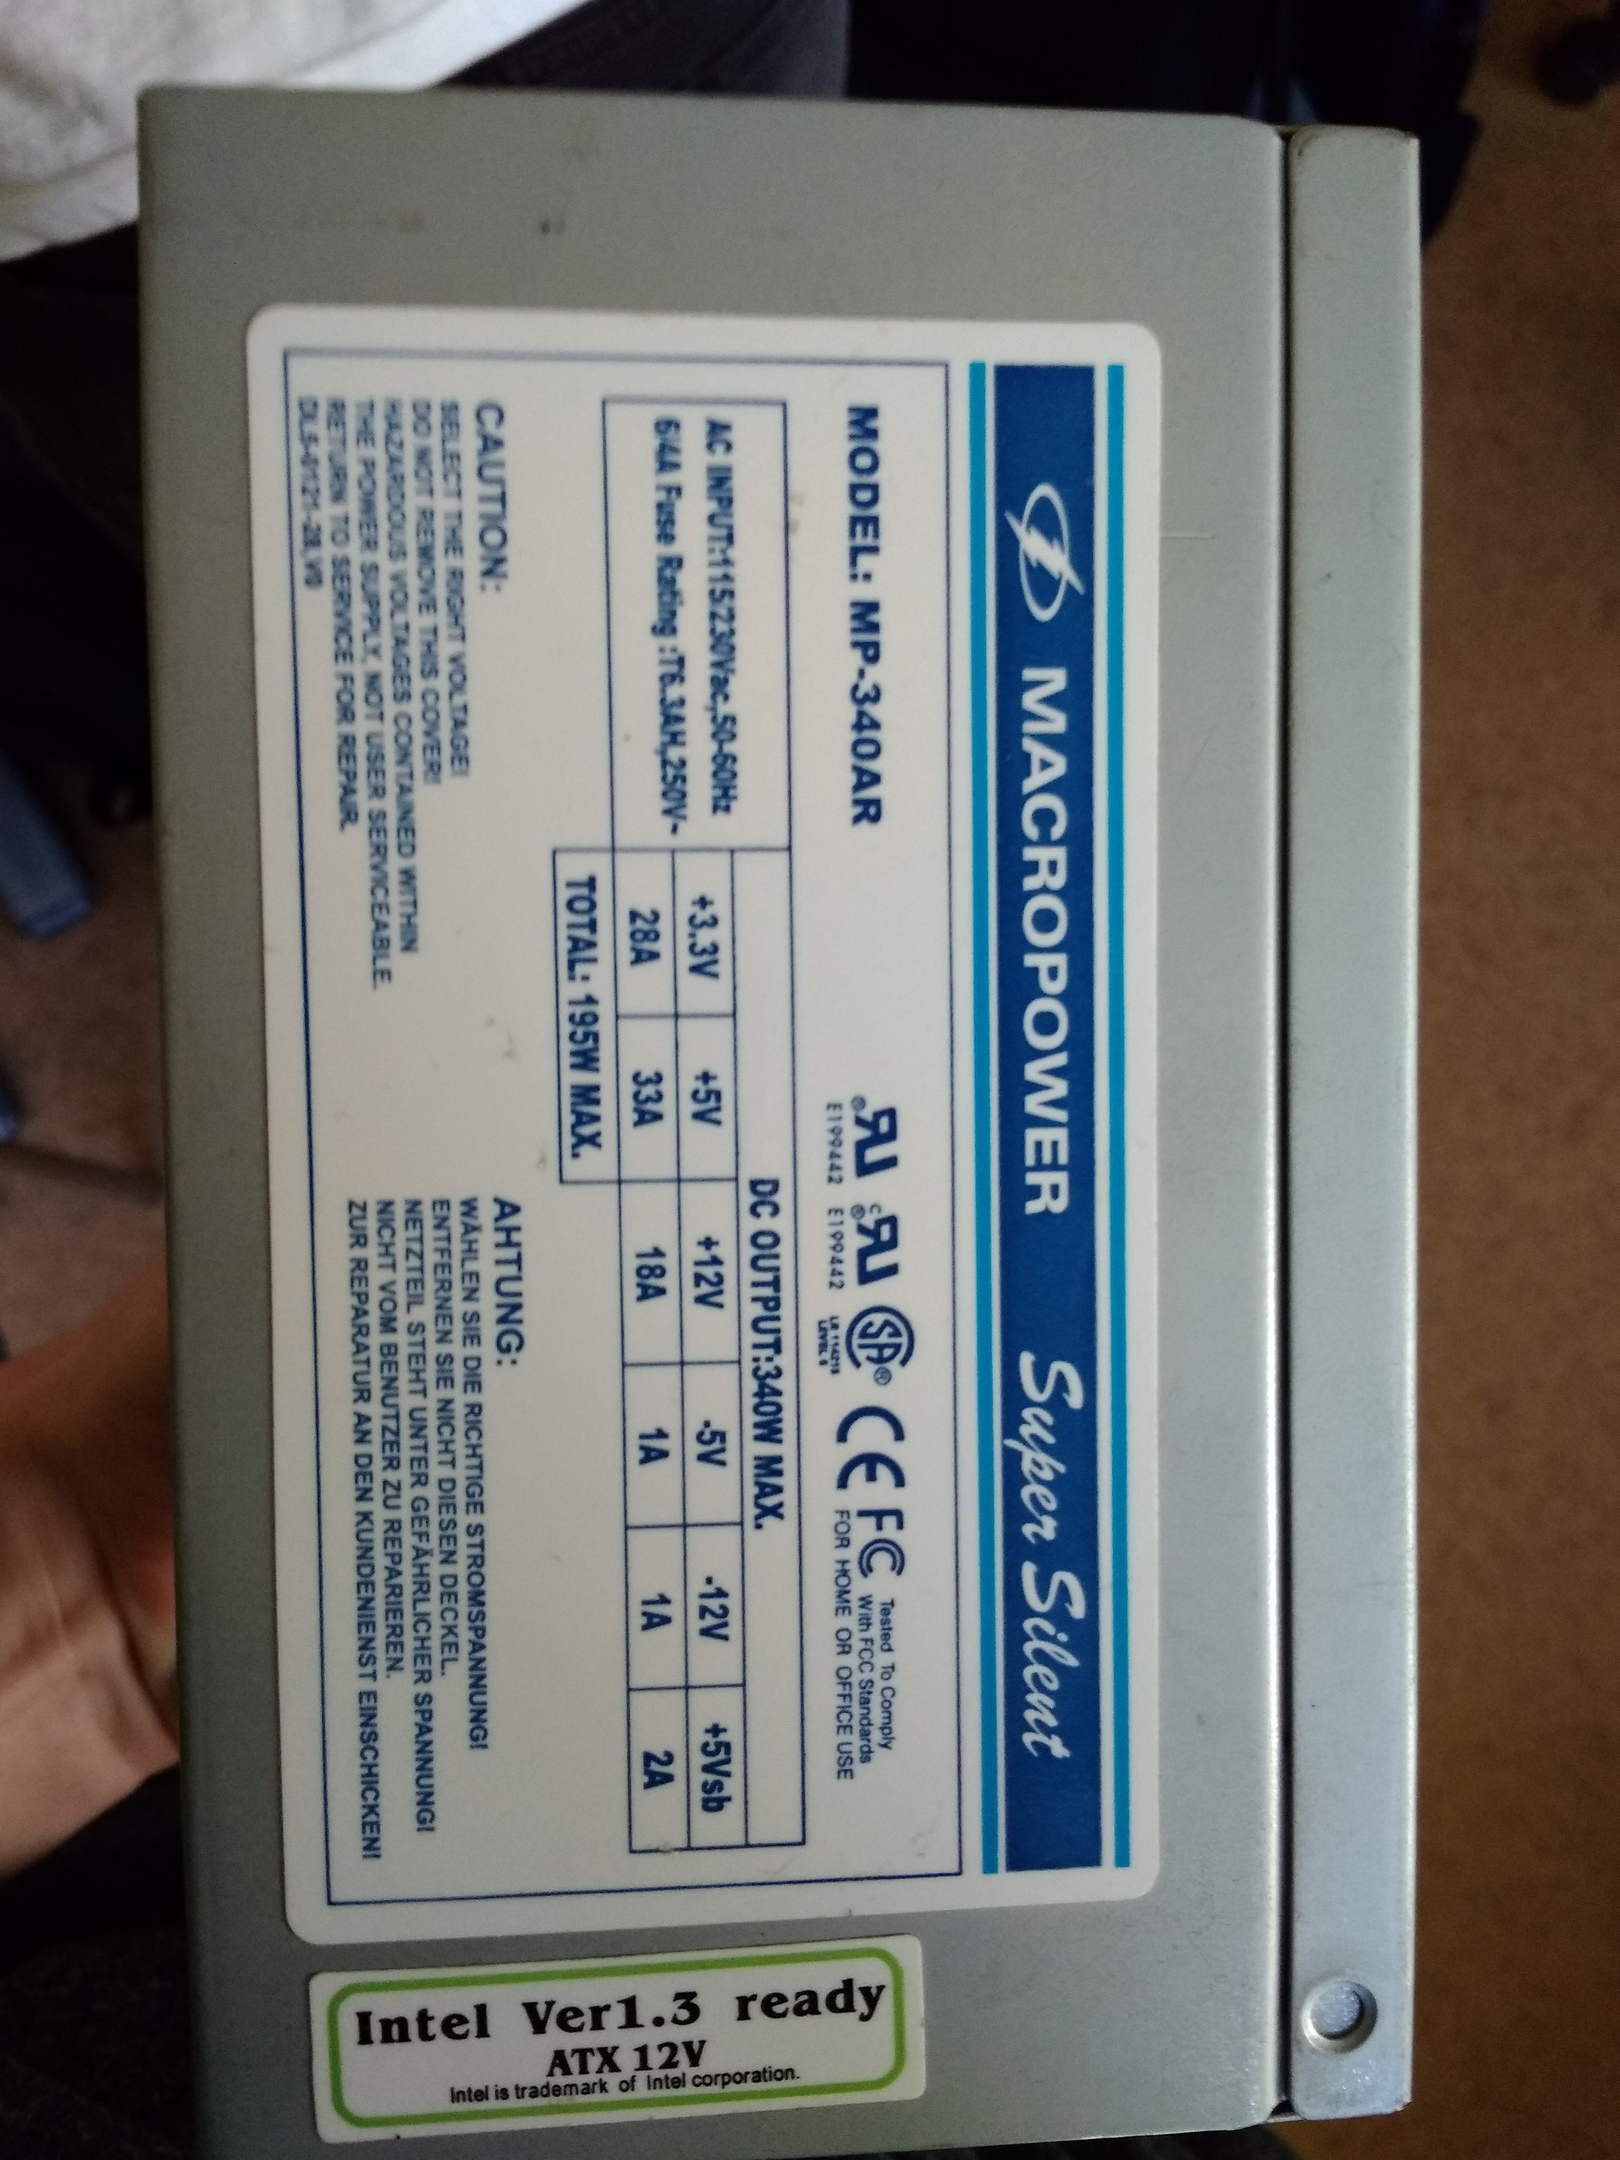
\includegraphics[scale=0.1]{power.jpg} 
\end{figure}
\subsubsection{Характеристики}
\begin{table}[H]
\centering
\begin{tabular}{|l|l|}
\hline
Характеристика & Значение \\
\hline
Форм-фактор & ATX \\
Входное напряжение & 50/60 Hz, 230 V \\
Мощность & 340 W max. \\
Разъёмы & 1x 20+4pin, 1x 4pin, 8x molex, 2x floppy, 1x SATA \\
\hline
\end{tabular} 
\end{table}

\section{Вывод}
В ходе лабораторной работы при разборке ПК на составные части и обратной сборке, мы изучили все его компоненты и занесли их в сводную таблицу, определив их основные характеристики.

Данная работа углубила наши знания в области строения ПК. Полученный опыт в будущем пригодится при ремонте ПК, его сборке или при покупке комплектующих.

\end{document}